\documentclass[captions=tableheading]{scrartcl}

\usepackage{amsmath}
\usepackage{amssymb}
\usepackage[utf8]{inputenc}
\usepackage[T1]{fontenc}
\usepackage{lmodern}
\usepackage{ngerman}
\usepackage{geometry}
\usepackage{graphicx}
\usepackage{wrapfig}
\usepackage{caption}
\usepackage{wasysym}
\usepackage[separate-uncertainty=true]{siunitx}
\usepackage{picinpar}
\usepackage{tikz}
\usepackage{float}
\usepackage{booktabs}

\renewcommand{\figurename}{Abb.}
\usepackage[
	colorlinks=true,
	urlcolor=blue,
	linkcolor=black
]{hyperref}


%Hier Titel und so
\newcommand{\versuchnummer}{V60} 
\newcommand{\versuchname}{Der Diodenlaser} 
\newcommand{\versuchdatum}{23.01.2017} 


\title{Versuch \versuchnummer\\ \versuchname}
\subtitle{Physikalisches Fortgeschrittenenpraktikum}
\author{Robert Rauter und Björn Lindhauer}
\date{\versuchdatum} 
\begin{document}
\begin{titlepage}
{\large \versuchdatum}
\vspace{7cm}
\begin{center}
\textbf{\huge Versuch \versuchnummer}\\\vspace{0.5cm}
\textbf{\huge \versuchname}\\
\vspace{0.2cm}
\textbf{Physikalisches Fortgeschrittenenpraktikum}\\
\vspace{9cm}

{\Large Robert Rauter \ \ \hspace{1.5cm} und \hspace{1.5cm} Björn Lindhauer}\\
{ \url{robert.rauter@tu-dortmund.de} \ \ \hspace{2cm} \url{bjoern.lindhauer@tu-dortmund.de}}
\end{center}
\end{titlepage}
\section{Einleitung}

\section{Theoretische Grundlagen}

\section{Aufbau}

\subsection{Justierung des Strahlengangs}
Zur Justierung des Strahlengangs wird eine Laserdetektionskarte in den Strahlengang gehalten und eine Videokamera auf die Photozelle gerichtet. \\
Zur Justierung des Strahlenganges sind zwei Drehschrauben am Diodenlaser vorhanden, jeweils für die horizontale und die vertikale Justierung.
 
\subsection{Beobachtung der Rubidium-Resonanz}
In Abbildung \ref{fig:setup} ist das Setup zur Detektion der Rubidium-Fluoreszenz dargestellt.
\begin{center}
	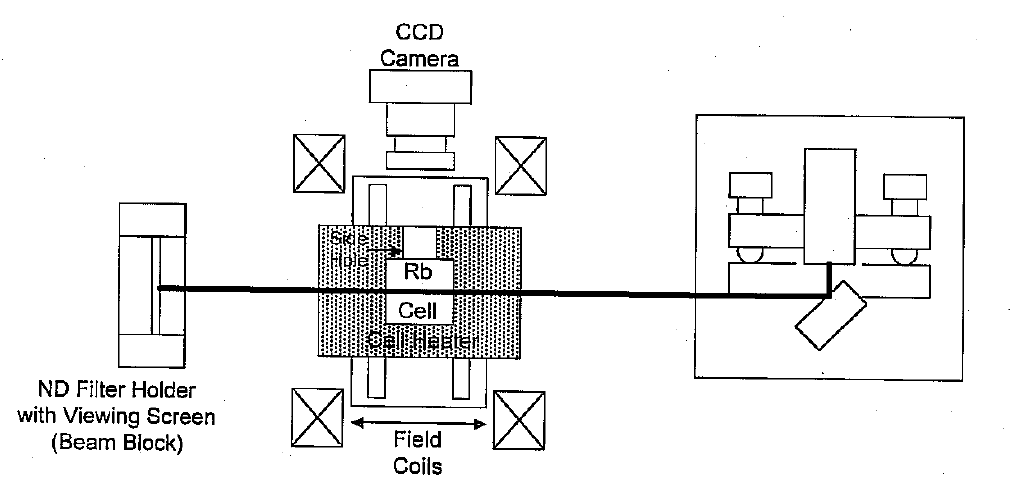
\includegraphics[width=10cm]{images/setup.png}
	\captionof{figure}{Setup zur Detektion von Rubidium-Fluoreszenz}
	\label{fig:setup}
\end{center}
Zur Detektion der Fluoreszenz wird der horizontale Winkel des Gitters schrittweise angepasst. Die Feinabstimmung wird durch eine Anpassung der Piezospannung erreicht. Im Falle einer Resonanz kann diese mit der Kamera und des Oszilloskop detektiert werden. \\

\section{Durchführung}

\subsection{Justierung des Strahlengangs}
Mithilfe einer Kamera kann das Verhalten des Strahls bei Variation der Stromstärke beobachtet werden. Unterhalb des Grenzwertes der Stromstärke verhält sich der Diodenlaser wie eine LED, d.h. es kommt zu spontaner Emission. Ein Bild es entstehenden Signals ist in Abbildung \ref{fig:led} zu sehen.
\begin{center}
	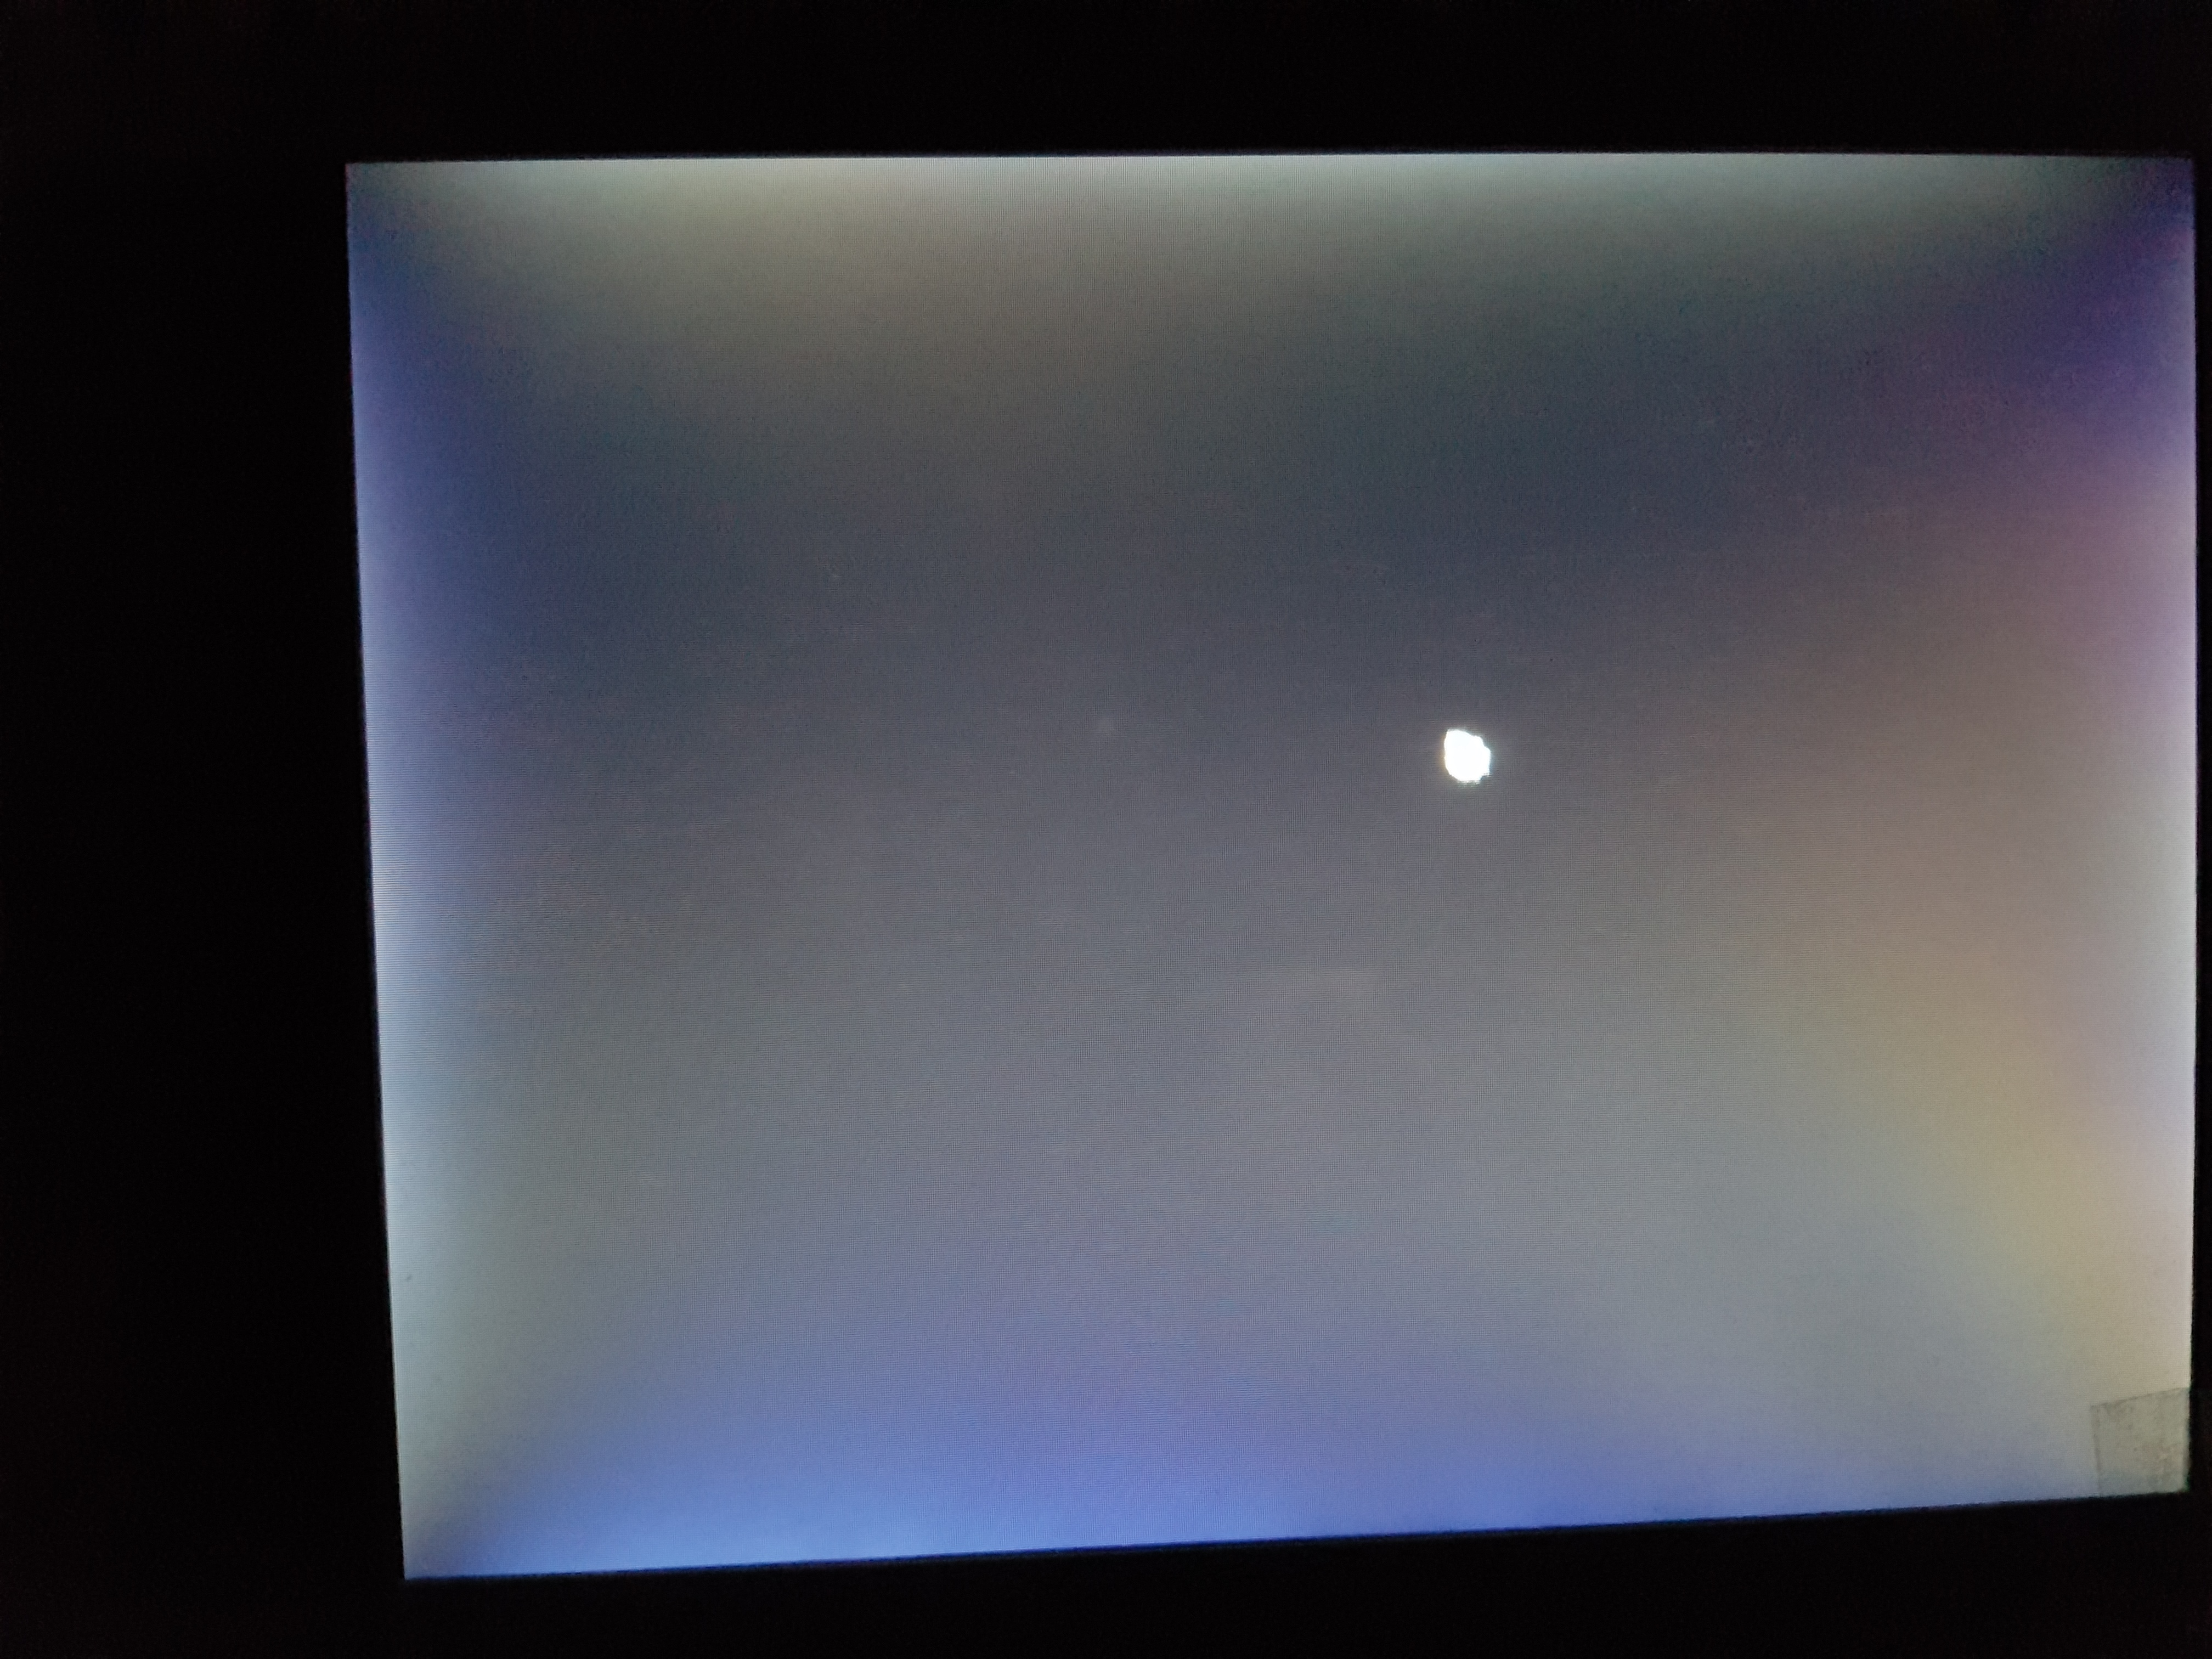
\includegraphics[width=10cm]{images/led_spot.jpg}
	\captionof{figure}{Beobachtetes Ausgangssignal des Diodenlasers unterhalb der Grenzstromstärke}
	\label{fig:led}
\end{center}
Wird der Grenzwert der Stromstärke überschritten, tritt eine deutliche Erhöhung der Strahlintensität auf, wie es in Abbildung \ref{fig:over_threshold} zu sehen ist. 
\begin{center}
	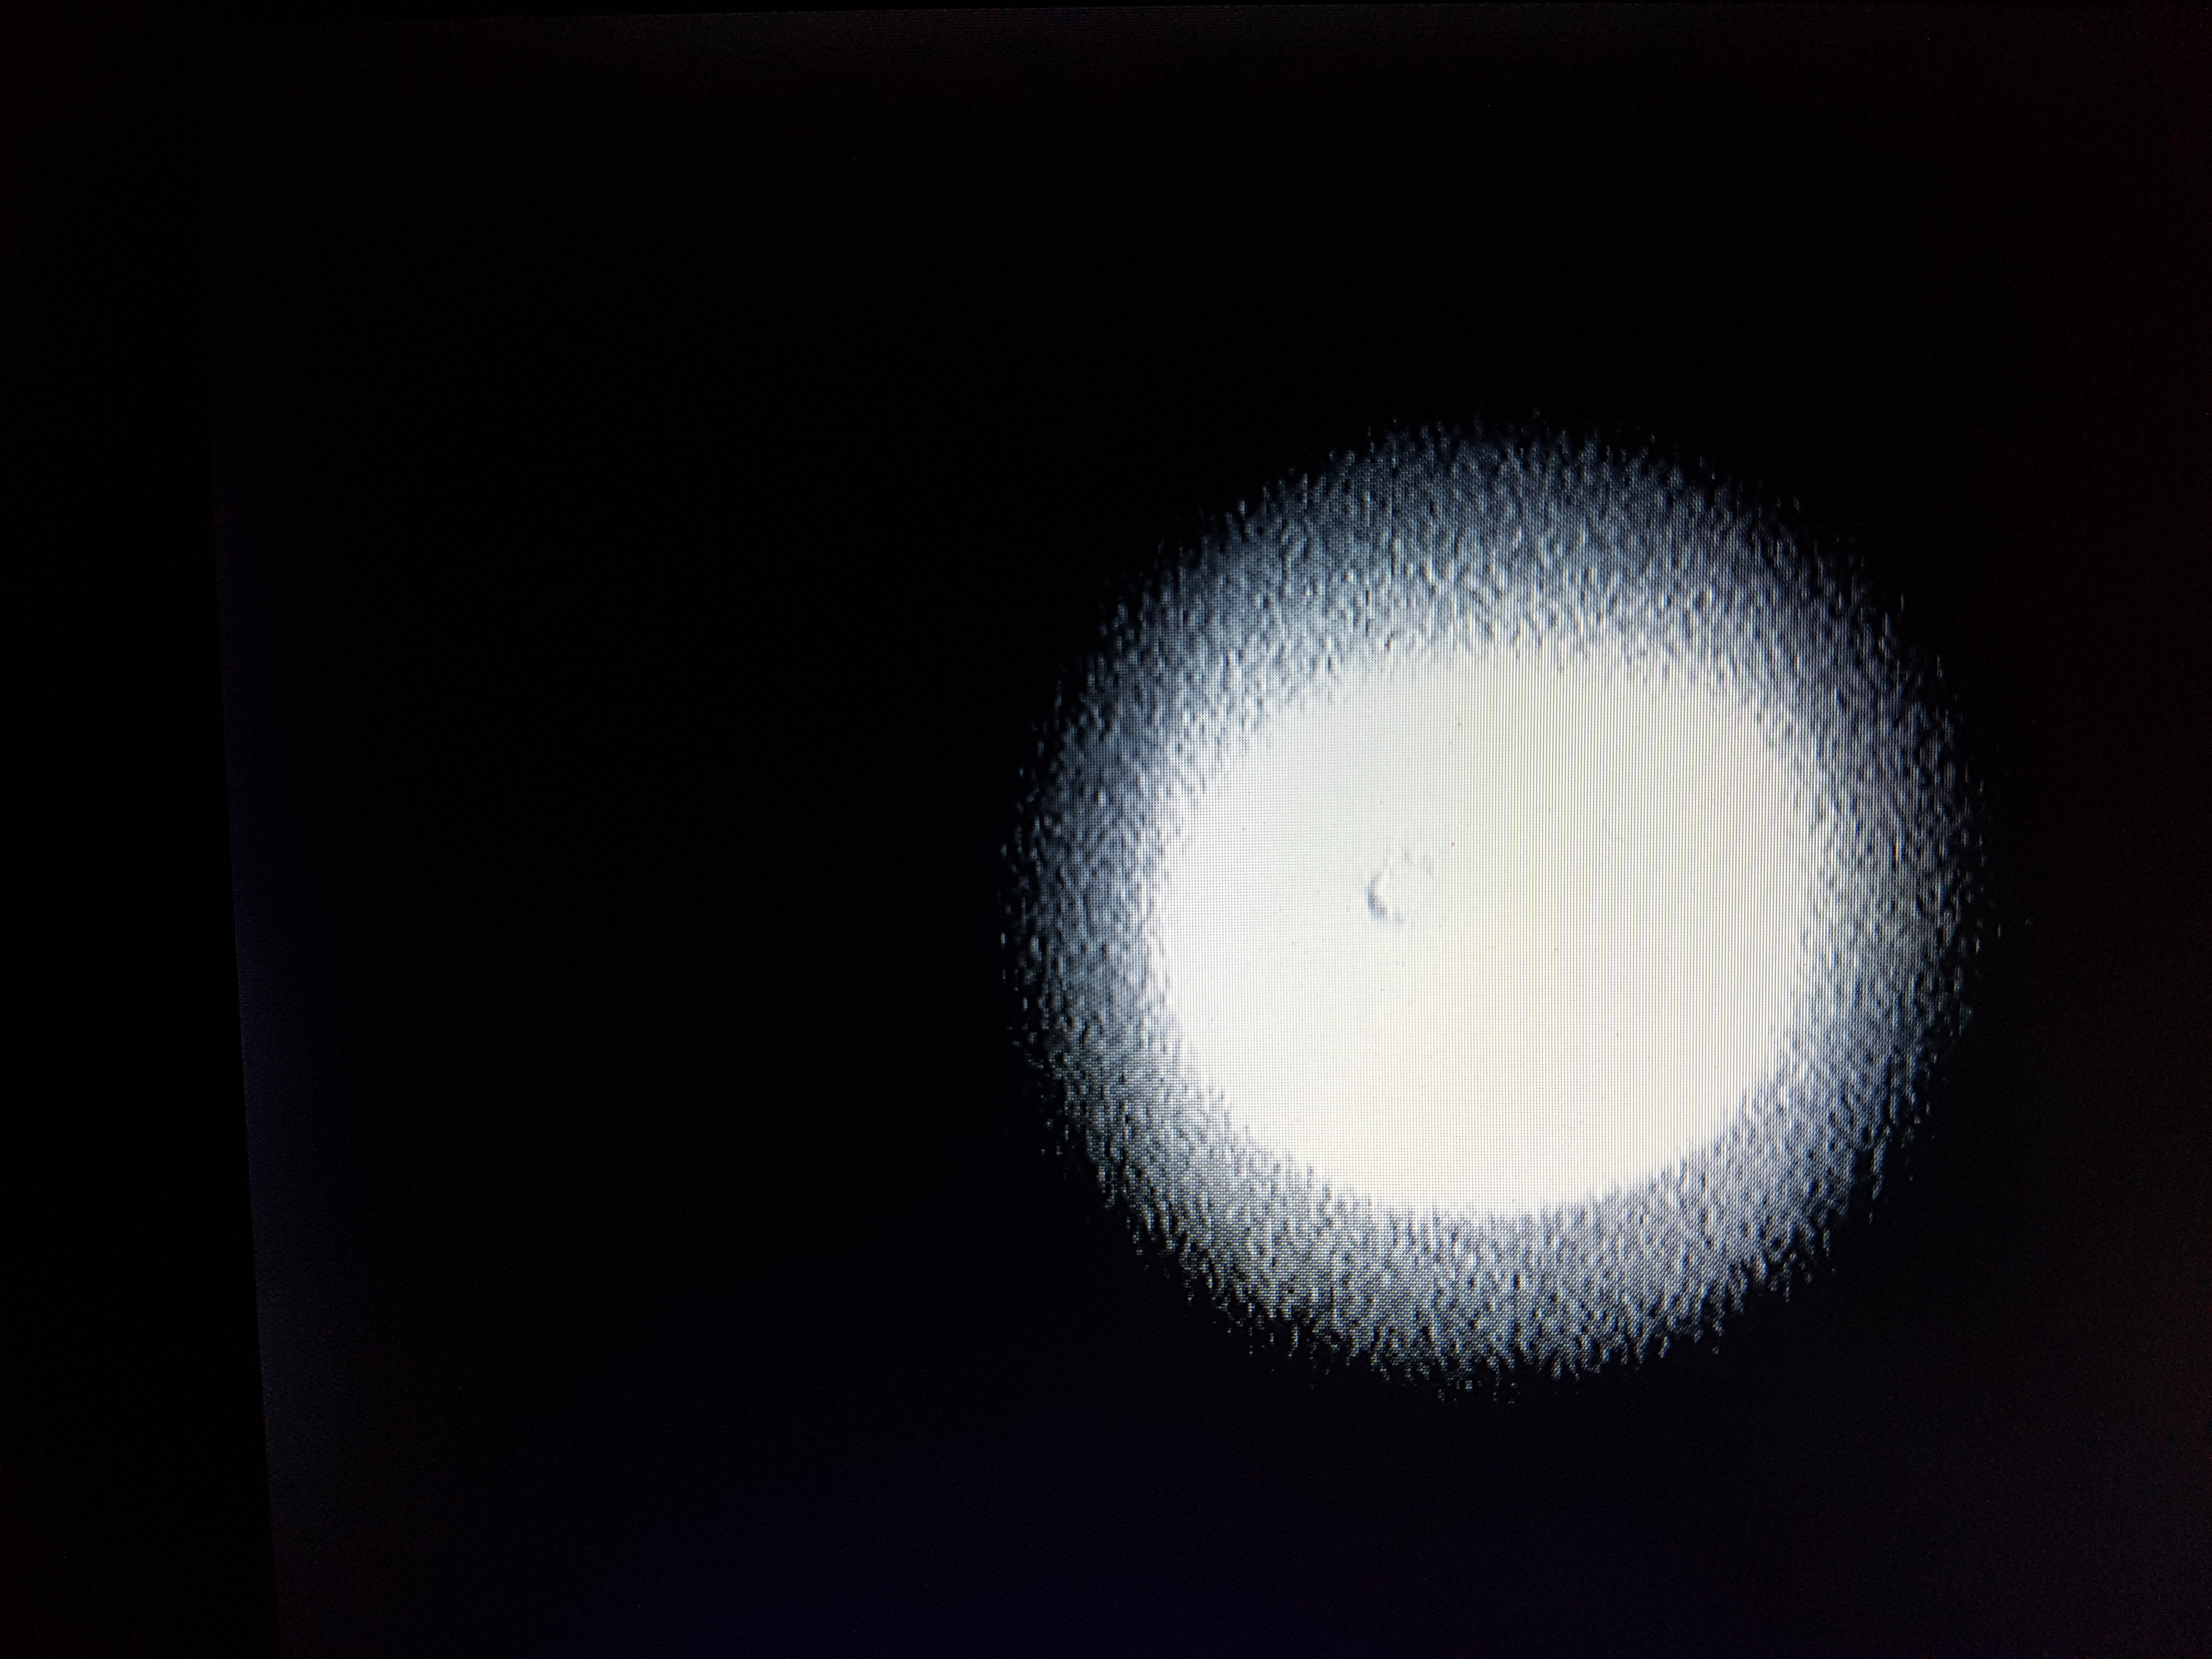
\includegraphics[width=10cm]{images/over_threshold.jpg}
	\captionof{figure}{Beobachtetes Ausgangssignal des Diodenlaser oberhalb der Grenzstromstärke}
	\label{fig:over_threshold}
\end{center}

\subsection{Beobachtung der Rubidium-Resonanz}
Mithilfe des im Kapitel 3 beschriebenen Aufbaus kann die Rubidium-Resonanz mittels einer Kamera beobachtet werden. Dies ist in Abbildung \ref{fig:resonanzbild} abgebildet.
\begin{center}
	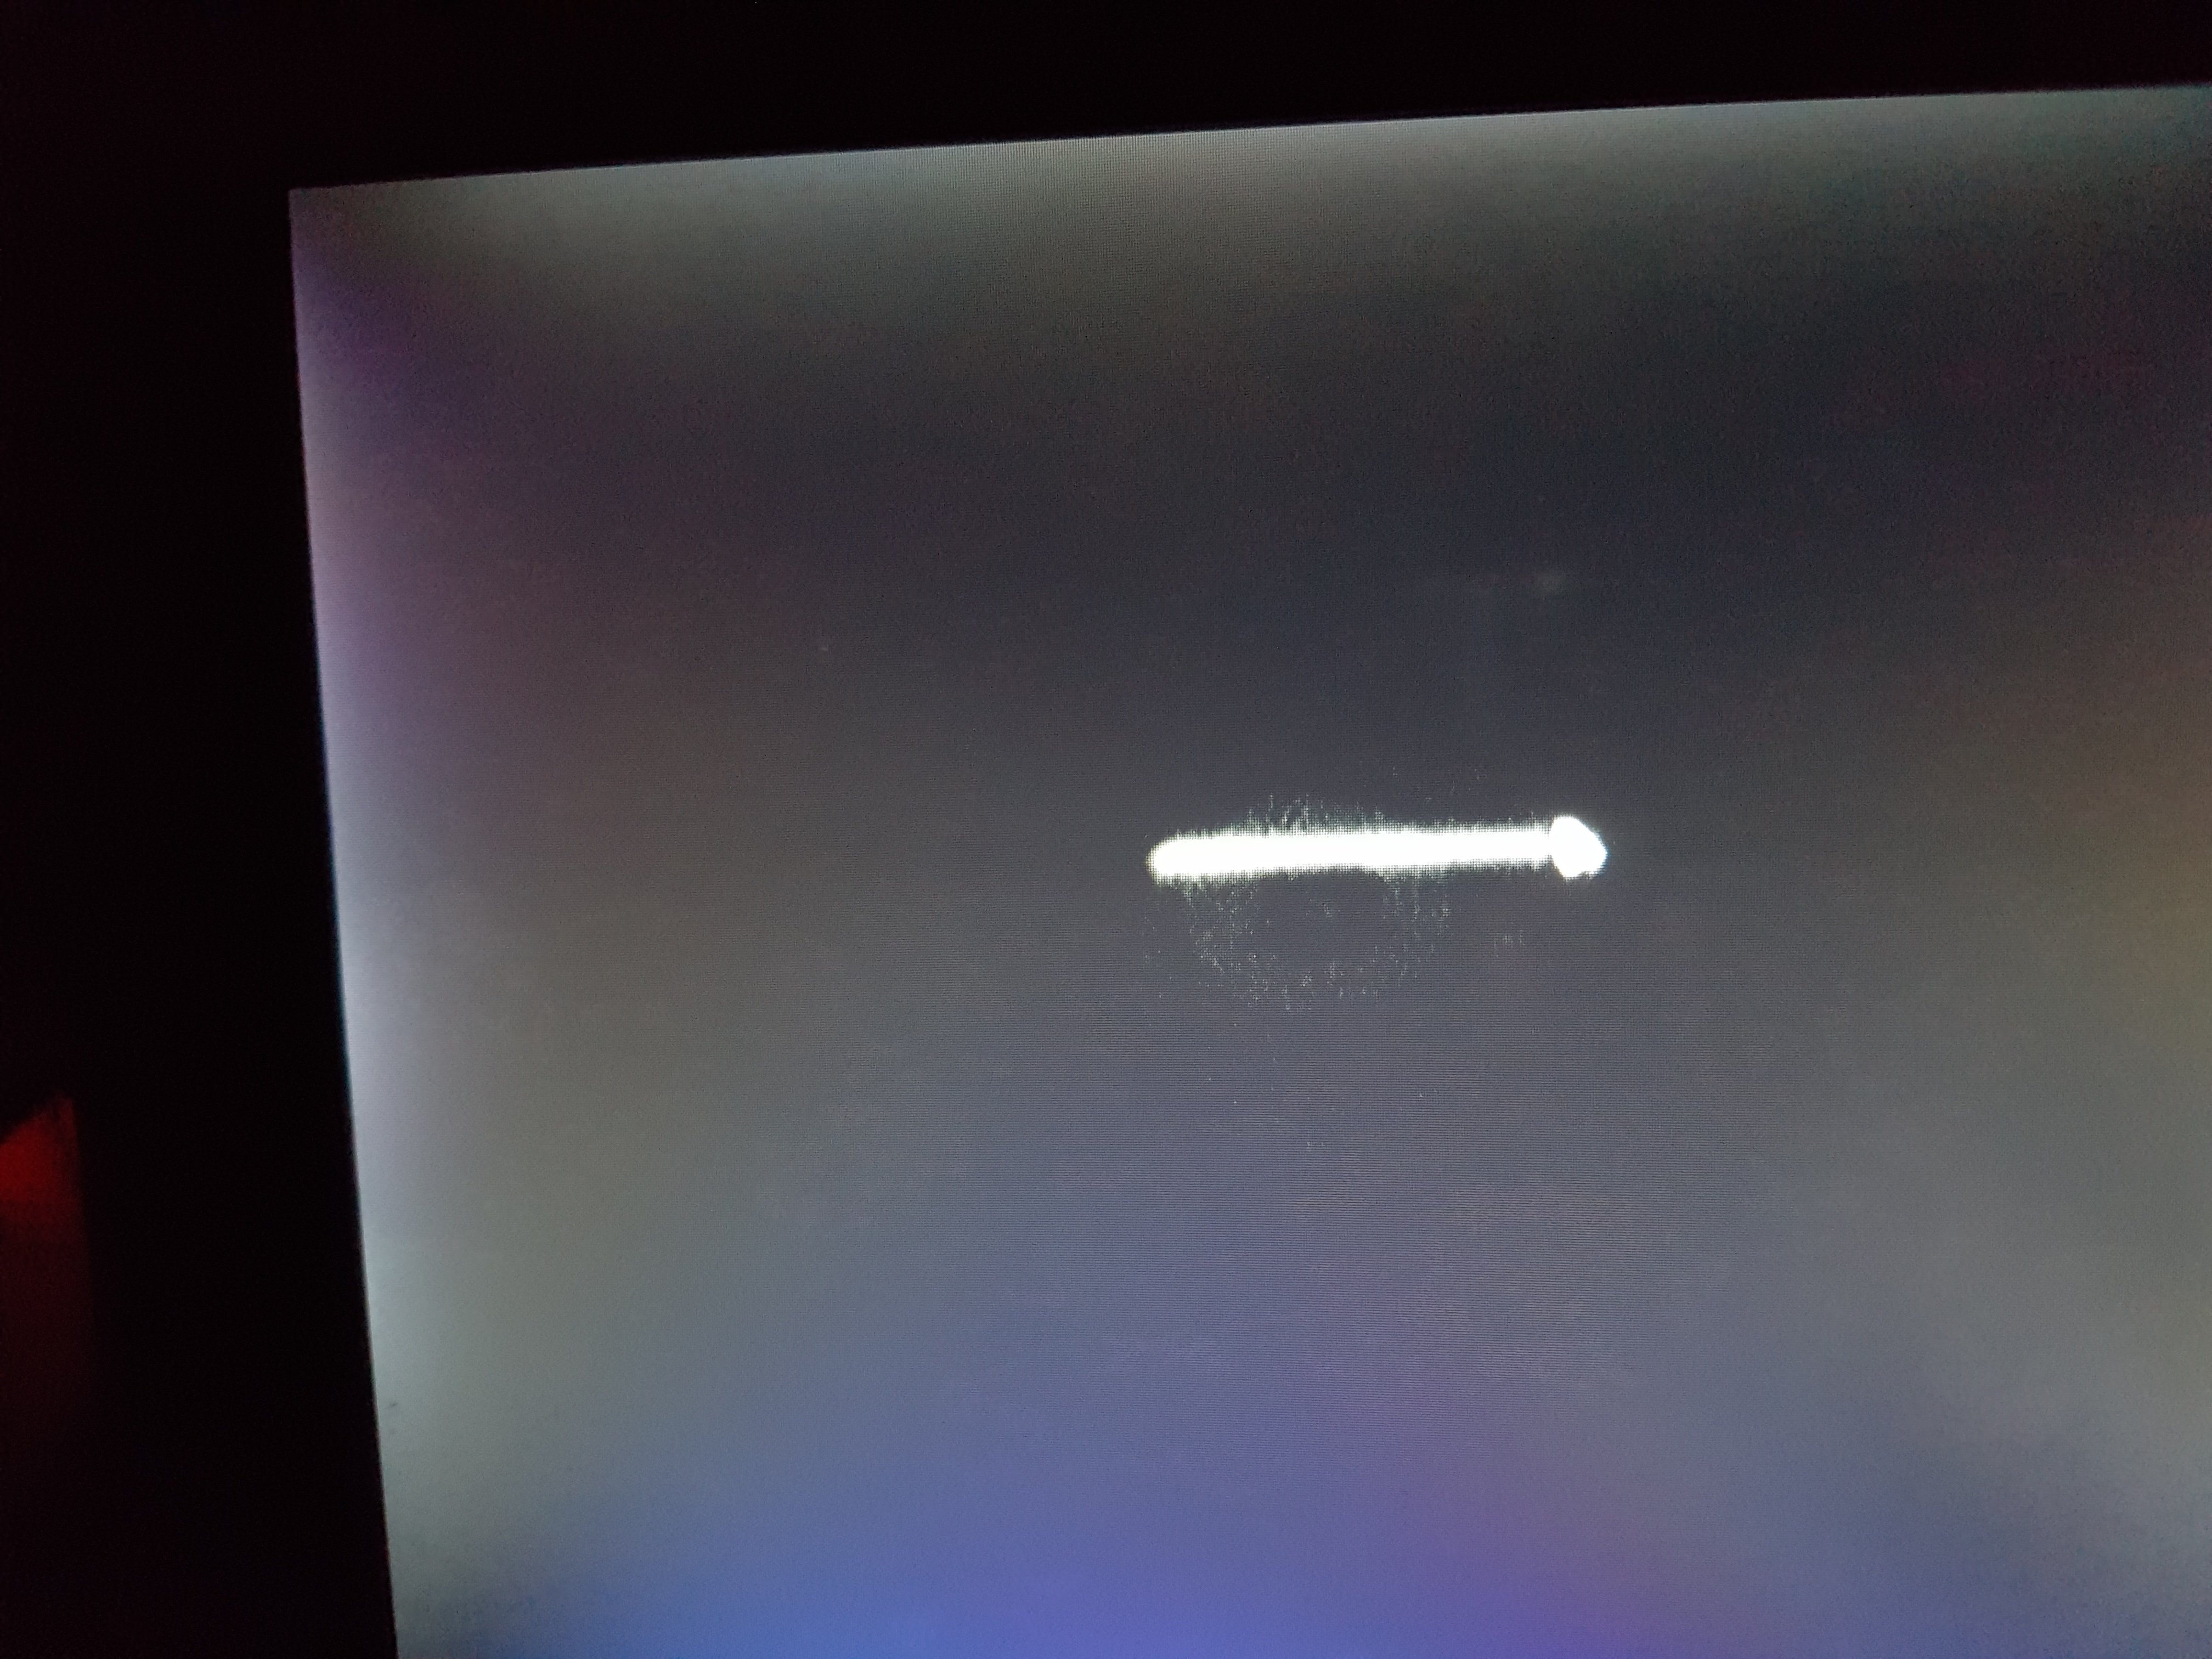
\includegraphics[width=10cm]{images/resonanz_bild.jpg}
	\captionof{figure}{Mit Kamera detektiertes Resonanzsignal}
	\label{fig:resonanzbild}
\end{center}
Um die Intensität zu verringern, wird ein Dämpfungsglied in den Strahlengang gestellt. Das Signal der Photodiode wird mithilfe eines Photodetektors detektiert und auf einem Oszilloskop dargestellt. 
\begin{center}
	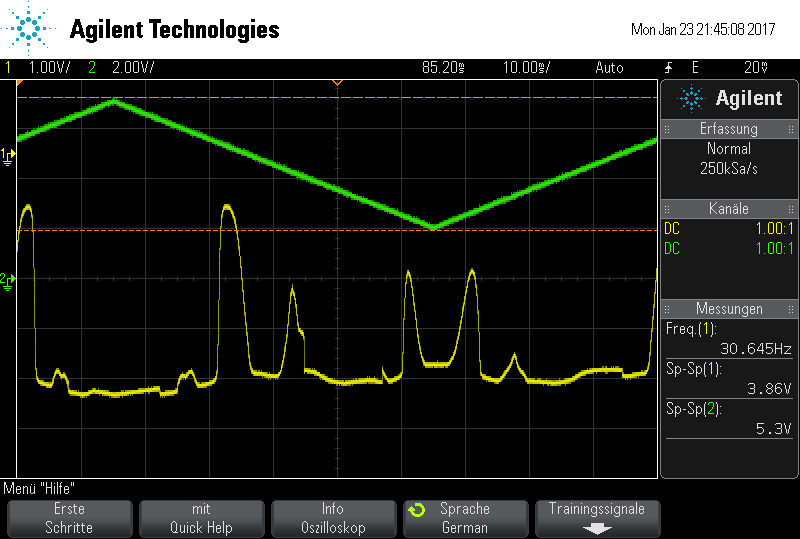
\includegraphics[width=10cm]{images/scope_22.png}
	\captionof{figure}{Resonanzspektrum von Rubidium}
	\label{fig:resonanz}
\end{center}
Das grüne Dreiecksignal ist die Spannung, die am Piezoelement anliegt, welches die Orientierung des Gitters bestimmt und somit die Frequenzen durchscannt. Das gelbe Signal zeigt die Absorptionspeaks der Photozelle, die durch den Rubidium-Dampf erzeugt werden.

\subsection{Bereinigung des Resonanzsignals}
Zur Bereinigung des Resonanzsignals von z.B. der Spannungsmodulation des Piezokristalles, wird mithilfe der Differenzspannungsmethode der Hintergrund des Signals entfernt. In Abbildung \ref{fig:resonanzlinien} ist dabei das Absorptionssignal ohne Hintergrundbereinigung dargestelt, in Abbildung \ref{fig:resonanzlinien_mh} das finale Signal ohne Hintergrund.
\begin{center}
	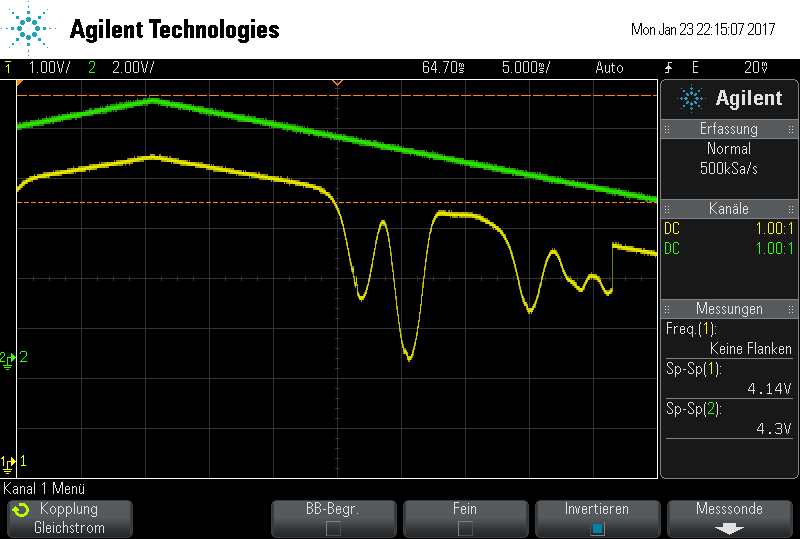
\includegraphics[width=10cm]{images/resonanz.png}
	\captionof{figure}{Resonanzlinien der Rubidium-Probe, mit Hintergrund-Intensität}
	\label{fig:resonanzlinien}
\end{center}

\begin{center}
	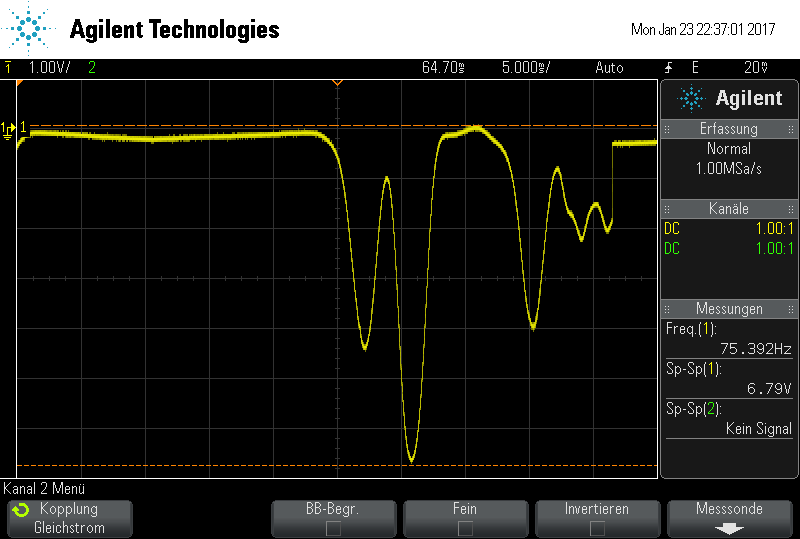
\includegraphics[width=10cm]{images/resonanz_bereinigt.png}
	\captionof{figure}{Um Hintergrund bereinigte Resonanzlinien der Rubidium-Probe}
	\label{fig:resonanzlinien_mh}
	\end{center}

\section{Diskussion}

\section{Quellen}
{[1]} Physikalisches Praktikum, TU Dortmund: \\
\textit{Versuchsanleitung zu Versuch 60: Der Diodenlaser} \\
http://129.217.
224.2/HOMEPAGE/PHYSIKER/MASTER/SKRIPT/V60.pdf (letzte Version vom 24.01.2017, 16:00)\\

\end{document}